\documentclass[letterpaper,11pt]{article}
\usepackage[spanish]{babel}
\usepackage[utf8]{inputenc}
\usepackage{graphicx}
\usepackage{amsfonts,amsmath,amssymb,float, amsthm,mathrsfs}  
\usepackage[right=4.5cm,left=2cm,top=3cm,bottom=3cm,headsep= 0.7cm,footskip=0.5cm]{geometry}
\usepackage{enumerate}
\usepackage{wrapfig} 
\usepackage[rflt]{floatflt} 
\usepackage{framed}
%\usepackage[most]{tcolorbox}
\usepackage[dvipsnames]{xcolor}
\colorlet{shadecolor}{green!20}
\setlength\FrameSep{0.5ex}
\usepackage{thmtools}
\usepackage{esint}
\usepackage{cancel}
\usepackage{listings} 
\usepackage{pstricks, caption}
\usepackage[colorlinks]{hyperref}
\usepackage{csquotes}
\usepackage{fullpage}
\usepackage{enumitem}
\usepackage{etoolbox}
\usepackage{tikz}
\usepackage{tikz-3dplot}
\tdplotsetmaincoords{80}{70}
\usetikzlibrary{decorations.markings}
\usetikzlibrary{arrows,babel}
\usepackage[font=small]{caption}
\usepackage{scalerel} %\scaleto{text}{size}
\usepackage{subfigure}
\usepackage{fancyhdr}
\usepackage{comment}
\usepackage{marginnote}
\usepackage{tensor}
\usepackage{cleveref}
\newcommand{\dbar}{\mathchar'26\mkern-12mu d}
\renewcommand*{\marginnotevadjust}{-0.1cm}
\renewcommand*{\marginfont}{\footnotesize}
\setlength{\headheight}{15pt}
\addtolength{\topmargin}{-14.49998pt}
\setlength{\headsep}{15pt}
\setlength{\footskip}{14.49998pt}
\decimalpoint
\newcommand{\grad}{^\circ}
\newlength{\drop}
\DeclareMathOperator{\sign}{sgn}
\DeclareMathOperator{\Log}{Log}
\providecommand{\norm}[1]{\lVert#1\rVert}

\let\cancelorigcolor\CancelColor% Just for conveniency...

\newcommand{\CancelTo}[3][]{%
  \ifblank{#1}{}{%
    \renewcommand{\CancelColor}{#1}%
  }
  \cancelto{#2}{#3}% 
}


\begin{document}

\pagestyle{plain}

\begin{flushleft}\vspace{-2cm}
Departamento de Física \\
Facultad de Cs. Físicas y Matemáticas\\
Universidad de Concepción
\end{flushleft}

\begin{flushright}\vspace{-1.5cm}
\textbf{Tópicos en Relatividad General} 
\end{flushright}



\rule{\linewidth}{0.1mm}

\begin{center}
\textbf{\LARGE Semana 4}
\end{center}

\begin{flushleft}
\textbf{Nombre:} Alejandro Saavedra San Martín. \\
\textbf{Profesor:} Guillermo Rubilar Alegría.
\end{flushleft}

\section*{Órbitas ligadas no-circulares}

Si $h > 2 \sqrt{3}$, $\tilde{V}(r_B) < k^2 < \tilde{V}(r_A)$ y $k < 1$, existen órbitas ligadas, cuyas coordenadas radiales varían entre $r_{\text{mín}}$ y $r_{\text{máx}}$, con $\tilde{V}(r_{\text{mín}}) = \tilde{V}(r_{\text{máx}}) = k^2$, ver figura \ref{fig:Potential}. 

\begin{figure}[H] 
    \centering
    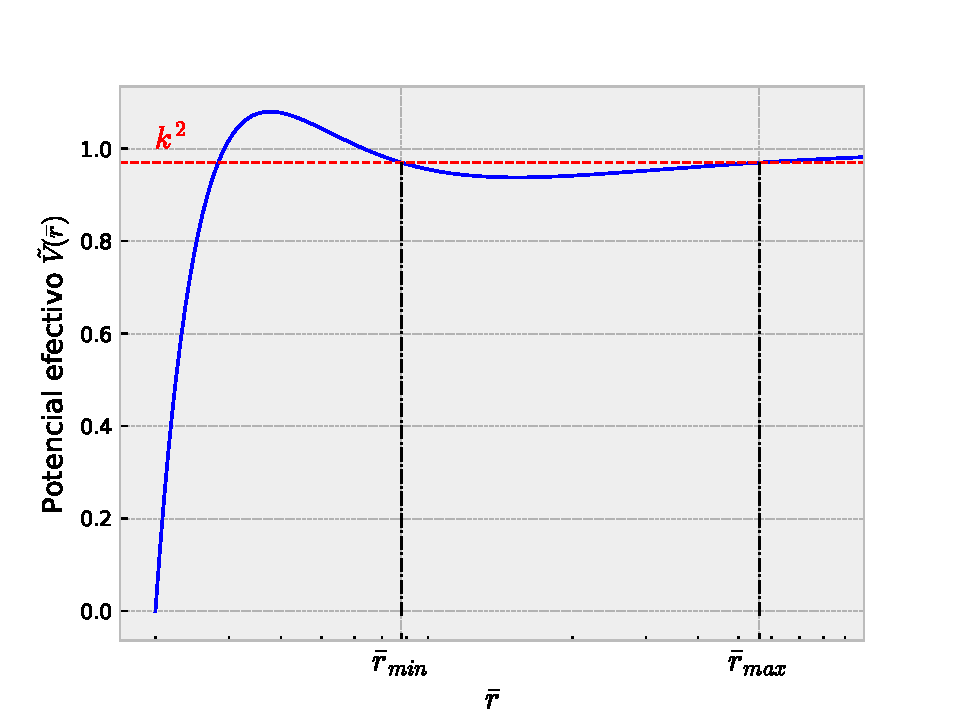
\includegraphics[scale = 0.7]{Potencial_Efectivo_orbita-ligada}
    \caption{Potencial efectivo para órbitas ligadas.}
    \label{fig:Potential}
\end{figure}

Para analizar la forma de la trayectoria consideremos  la coordenada radial en términos de la angular, $r = r(\varphi)$. Por regla de la cadena,
\begin{equation}
\dot{r} = \frac{dr}{d\varphi} \frac{d\varphi}{d\tau} = r' \dot{\varphi},
\end{equation}

donde $r' := dr/d\varphi$. Como $hmc = r^2 \sin\theta \dot{\varphi} = r^2 \dot{\varphi}$, 
\begin{equation}
hmc = r^2 \frac{\dot{r}}{r'}.
\end{equation}

Así,
\begin{equation} \label{eq:r-derivative}
\dot{r} = \frac{hmc}{r^2} r'.
\end{equation}

Derivando con respecto a $\tau$ la ecuación \eqref{eq:r-derivative}, obtenemos
\begin{align}
\ddot{r} &= - \frac{2 hmc}{r^3} r' \dot{r} + \frac{hmc}{r^2} r'' \dot{\varphi} \nonumber \\
&= - \frac{2 hmc}{r^3} r' \left( \frac{hmc}{r^2} r' \right) + \frac{hmc}{r^2} r'' \left( \frac{hmc}{r^2} \right) \nonumber \\
&= - 2 h^2m^2c^2 \frac{r'\,^2}{r^5} + h^2m^2c^2 \frac{r''}{r^4}\nonumber  \\
&= \frac{h^2m^2c^2}{r^2} \left( - \frac{2}{r} r'\,^2 + r'' \right). \label{eq:r-second-derivative}
\end{align}

Al igual que en el caso newtoniano, definimos la variable auxiliar
\begin{equation} \label{eq:def-u}
u := \frac{1}{r}.
\end{equation}

Derivando con respecto a $\varphi$:
\begin{equation}
u' = - \frac{r'}{r^2} = - u^2 r'.
\end{equation}

Así,
\begin{equation} \label{eq:derivative-u}
r' = - \frac{1}{u^2} u'.
\end{equation}

Luego, la segunda derivada es
\begin{align}
u'' &= \frac{d}{d\varphi} (-u^2 r') \nonumber \\
&= -2 u u' r' - u^2 r'' \nonumber \\
&=  -2 u u' \left(- \frac{u'}{u^2} \right) - u^2 r'' \nonumber \\
&= 2 \frac{u'\,^2}{u} - u^2 r''.
\end{align}

Despejando $r''$:
\begin{equation} \label{eq:2nd-derivative-u}
r'' = \frac{2}{u^3} u'\,^2 - \frac{1}{u^2} u''.
\end{equation}

En el documento de la semana 3 encontramos que la dinámica de la coordenada $r$ está determinada por la ecuación
\begin{equation}
\dot{r}^2 = k^2c^2 - c^2 \left(1 - \frac{2m}{r}\right)\left(1 + \frac{h^2m^2}{r^2}\right).
\end{equation}

Usando \eqref{eq:r-derivative}, \eqref{eq:def-u} y \eqref{eq:derivative-u}, encontramos que 
\begin{align}
\frac{h^2m^2\cancel{c^2}}{r^4} r'\,^2 &= k^2\cancel{c^2} - \cancel{c^2} \left(1 - \frac{2m}{r} \right)\left(1 + \frac{h^2m^2}{r^2}\right) \\
h^2m^2u^4 \left(-\frac{1}{u^2} u' \right) &= k^2 - (1-2mu)(1+h^2m^2u^2). 
\end{align} 

Entonces,
\colorlet{shadecolor}{green!20}
\begin{shaded}
\begin{equation} \label{eq:motion-u'}
h^2m^2u'\,^2 - k^2 + (1-2mu)(1+h^2m^2u^2) = 0.
\end{equation}
\end{shaded}

Derivando con respecto a $\varphi$ la ecuación \eqref{eq:motion-u'}:
\begin{align}
2h^2m^2u' u'' - 2mu' (1+h^2m^2u^2) + (1-2mu)(2h^2m^2uu') &= 0 \\
2h^2m^2u' u'' - 2mu' - 2h^2m^3u^2u' + 2h^2m^2uu' - 4h^2m^3u^2u' &= 0 \\
h^2m^2 u' u'' - m u' - 3h^2m^3 u^2 u' + h^2m^2 u u' &= 0 \\
h^2m^2 u' u'' + h^2m^2 u u' &=  m u' + 3h^2m^3 u^2 u' \\
 u' u'' +  u u' &=  \frac{1}{h^2 m} u' + 3m u^2 u'.
\end{align}

Ahora, si no consideramos órbitas circulares, ésto es $r$ no constante con $u' \neq 0$, obtenemos que
\begin{shaded}
\begin{equation} \label{eq:motion-u''}
u'' + u = \frac{1}{h^2m} + 3mu^2.
\end{equation}
\end{shaded}

Si definimos la variable adimensional
\begin{equation}
w := h^2m u.
\end{equation}

La ecuación \eqref{eq:motion-u''} puede escribirse como
\begin{align}
\frac{1}{h^2m} w'' + \frac{1}{h^2m} w &= \frac{1}{h^2m} + \frac{3m}{m^2h^4} w^2 \\
w'' + w &= 1 + \frac{3}{h^2} w^2.
\end{align}

Finalmente, si $\epsilon:= 3/h^2$, entonces 
\begin{shaded}
\begin{equation} \label{eq:motion-w''}
w'' + w = 1 + \epsilon w^2.
\end{equation}
\end{shaded}

El parámetro $\epsilon$ es pequeño (mucho menor que 1). En efecto, como $hmc = r^2 \dot{\varphi}$, 
\begin{equation}
\epsilon = \frac{3 m^2c^2}{r^4\dot{\varphi}^2} \approx \frac{3m^2c^2}{r^2 v_{\varphi}^2},
\end{equation}
donde $v_{\varphi} = r \dot{\varphi}$ es la velocidad tangencial. Si consideremos que los cuerpos están orbitando en campos débiles, por ejemplo en el sistema solar, de la mecánica newtoniana:
\begin{equation}
G \frac{\bar{m} M}{r^2} = \bar{m} \frac{v_{\varphi}^2}{r} \Rightarrow v_{\varphi}^2 \approx \frac{G M}{r} = \frac{mc^2}{r},
\end{equation}
con $\bar{m}$ la masa del cuerpo orbitando. Luego,
\begin{equation} \label{eq:epsilon}
\epsilon \approx 3 \frac{m^2}{r^2} \frac{c^2}{v_{\varphi}^2} \approx 3 \frac{m^2c^2}{r^2} \frac{r}{mc^2} = \frac{3m}{r} \ll 1. 
\end{equation}

En particular para Mercurio, se tienen los siguientes datos: \footnote{Datos sacados de \url{
https://physics.nist.gov/cuu/Constants/} y \url{https://nssdc.gsfc.nasa.gov/planetary/factsheet/mercuryfact.html}}
\begin{align}
G &= 6.67430 \times 10^{-11} \,\left[ \frac{m^3}{kg \,s^2} \right], \quad  c =  299 792 458 \,\left[ \frac{m}{s}\right], \quad  M_{\odot} = 1.988 \times 10^{30} \,[kg], \label{eq:mercury-data}\\
 r &= 57.909 \times 10^{9} \,[m]. 
\end{align}

Reemplazando los datos en \eqref{eq:epsilon}:
\begin{equation}
\epsilon \approx \frac{3 GM}{c^2r} =  \frac{3(6.67430 \times 10^{-11} ) ( 1.988 \times 10^{30})}{(299 792 458)^2( 57.909 \times 10^{9})} = 7.65 \times 10^{-8} \approx 10^{-7}.
\end{equation}

Por lo tanto, ocuparemos $\epsilon$ como parámetro perturbativo. 

Usando el método perturbativo, postulamos la siguiente expansión para la solución de \eqref{eq:motion-w''}:
\begin{equation}
w = w_0(\varphi) + \epsilon w_1(\varphi) + \epsilon^2 w_2(\varphi) + \mathcal{O}(\epsilon^3),
\end{equation}
donde $w_0$ es la solución no perturbada de
\begin{equation}
w_0'' + w_0 = 1,
\end{equation}
la cual corresponde a la ecuación diferencial ordinaria (EDO) de un oscilador armónico con término forzante constante, cuya solución es \footnote{En general la solución debe tener una fase inicial $ 1 + e \cos(\varphi - \varphi_0)$, pero se elige el sistema coordenado tal que $\varphi_0 = 0$.}
\begin{equation}
w_0(\varphi) = 1 + e \cos(\varphi).
\end{equation}

Reemplazando la solución perturbada en \eqref{eq:motion-w''}, obtenemos 
\begin{align}
w'' + w &= 1 + \epsilon w^2 \\
w_0'' + \epsilon w_1'' + w_0 + \epsilon w_1 + \mathcal{O}(\epsilon^2) &= 1 + \epsilon \left( w_0 + \epsilon w_1 + \mathcal{O}(\epsilon^2)\right)^2 \\
(w_0'' + w_0) + \epsilon (w_1'' + w_1)+ \mathcal{O}(\epsilon^2) &= 1 + \epsilon w_0^2 + \mathcal{O}(\epsilon^2) \\
1 + \epsilon(w_1'' + w_1)+ \mathcal{O}(\epsilon^2) &= 1 + \epsilon w_0^2 + \mathcal{O}(\epsilon^2).
\end{align}

Igualando los términos de primer orden en $\epsilon$, $w_1$ es solución de la EDO
\begin{align}
w_1'' + w_1 &= w_0^2 \nonumber \\
&= (1 + e\cos\varphi)^2  \nonumber\\
&= 1 + 2e \cos\varphi + e^2 \cos^2\varphi  \nonumber\\
&= 1 + 2e \cos\varphi + e^2 \left( \frac{1}{2} + \frac{1}{2} \cos(2\varphi) \right) \nonumber \\
&= \textcolor{red}{\left( 1 + \frac{e^2}{2}\right)} + \textcolor{blue}{2 e\cos\varphi} + \textcolor{green}{\frac{e^2}{2} \cos(2\varphi)}, \label{eq:EDO-w1}
\end{align}
donde se usó la identidad $\cos^2\varphi \equiv (1 + \cos(2\varphi))/2$.

Reconocemos la EDO de un oscilador forzado con términos forzantes: \textcolor{red}{constante}, \textcolor{blue}{resonante} y \textcolor{green}{periódico no resonante}. Por lo tanto, su solución general está dada por
\begin{equation}
w_1 = A + B \varphi \sin\varphi + C \cos(2\varphi).
\end{equation}

Reemplazando en la ecuación \eqref{eq:EDO-w1}:
\begin{align}
w_1'' + w_1 &= \left( 1 + \frac{e^2}{2}\right) + 2 e\cos\varphi + \frac{e^2}{2} \cos(2\varphi) \\
- B \varphi \sin(\varphi) + 2B \cos(\varphi) - 4C \cos(2\varphi) +  A + B \varphi \sin\varphi + C \cos(2\varphi) &= \left( 1 + \frac{e^2}{2}\right) + 2 e\cos\varphi + \frac{e^2}{2} \cos(2\varphi) \\
A + 2B\cos(\varphi) - 3C \cos(2\varphi) &= \left( 1 + \frac{e^2}{2}\right) + 2 e\cos\varphi + \frac{e^2}{2} \cos(2\varphi). 
\end{align}

Como las funciones $\cos(n\varphi)$, $n = 0,1,2,\dots$ son linealmente independientes, 
\begin{equation}
A = 1 + \frac{e^2}{2}, \quad B = e, \quad C = - \frac{e^2}{6}.
\end{equation}

Por lo tanto, la solución de la ecuación \eqref{eq:motion-u''} a primer orden en $\epsilon$ toma la forma:
\begin{equation} \label{eq:sol-u-perturbado-1}
u(\varphi) = \frac{1}{mh^2} \left[ 1 + e\cos\varphi + \epsilon\left[ \left( 1 + \frac{e^2}{2}\right) + e \varphi \sin\varphi - \frac{e^2}{6} \cos(2\varphi) \right] \right] + \mathcal{O}(\epsilon^2).
\end{equation}

Usando las expansiones en serie de Taylor para el coseno y seno:
\begin{align}
\cos(x) &= 1 - \frac{x^2}{2!} + \frac{x^4}{4!} - \cdots, \\
\sin(x) &= x - \frac{x^3}{3!} + \frac{x^5}{5!} - \cdots . 
\end{align}

Entonces,
\begin{align}
\cos(\epsilon \varphi) &= 1 + \mathcal{O}(\epsilon^2), \\
\sin(\epsilon \varphi) &= \epsilon \varphi + \mathcal{O}(\epsilon^3).
\end{align}

De esta forma podemos escribir 
\begin{align}
\cos \varphi + \epsilon \varphi \sin\varphi &= \textcolor{red}{1} \cdot \cos \varphi + \textcolor{blue}{\epsilon \varphi} \sin\varphi \nonumber \\
&= \textcolor{red}{\cos(\epsilon \varphi)} \cos \varphi + \textcolor{blue}{\sin(\epsilon \varphi)} \sin\varphi + \mathcal{O}(\epsilon^2)\nonumber \\
&= \cos(\epsilon \varphi - \varphi ) + \mathcal{O}(\epsilon^2)\nonumber \\
&= \cos[(1 - \epsilon)\varphi] + \mathcal{O}(\epsilon^2).
\end{align}

Análogamente,
\begin{align}
\epsilon \cos(2\varphi) &= \epsilon \cos(2\varphi - 2 \epsilon \varphi + 2\epsilon \varphi) \nonumber\\
&=  \epsilon \cos(2 (1 - \epsilon) \varphi + 2 \epsilon \varphi) \nonumber\\
&= \epsilon \{ \cos[2(1 - \epsilon)\varphi] \textcolor{red}{\cos(2\epsilon \varphi)} - \sin [2(1 - \epsilon)\varphi]\textcolor{blue}{\sin(2\epsilon \varphi)}\}\nonumber\\
&= \epsilon \{ \cos[2(1 - \epsilon)\varphi] \textcolor{red}{(1 + \mathcal{O}(\epsilon^2))} - \sin [2(1 - \epsilon)\varphi] \textcolor{blue}{(2\epsilon\varphi + \mathcal{O}(\epsilon^3))}\} \nonumber\\
&= \epsilon \cos[2(1-\epsilon)\varphi] + \mathcal{O}(\epsilon^2).
\end{align}

Luego, podemos expresar la solución \label{eq:sol-u-perturbado-2} de la siguiente forma:
\begin{align}
u(\varphi) &= \frac{1}{mh^2} \left[ 1 + e\cos\varphi + \epsilon \left( 1 + \frac{e^2}{2}\right) + e \epsilon \varphi \sin\varphi - \frac{e^2}{6} \epsilon \cos(2\varphi) \right] + \mathcal{O}(\epsilon^2) \nonumber\\
&= \frac{1}{mh^2} \left[ 1 + \epsilon \left( 1 + \frac{e^2}{2}\right) + e \textcolor{red}{(\cos\varphi +  \epsilon \varphi \sin\varphi)} - \frac{e^2}{6} \textcolor{blue}{\epsilon \cos(2\varphi)} \right] + \mathcal{O}(\epsilon^2) \nonumber\\
&= \frac{1}{mh^2} \left[ 1 + \epsilon \left( 1 + \frac{e^2}{2}\right) + e \textcolor{red}{\cos[(1-\epsilon)\varphi]} - \frac{e^2}{6} \textcolor{blue}{\epsilon \cos[2(1-\epsilon)\varphi]} \right] + \mathcal{O}(\epsilon^2) .
\end{align}

Por lo tanto, la solución a primer orden en $\epsilon$ puede escribirse como
\begin{shaded}
\begin{equation} \label{eq:u-solution-pertur}
u(\varphi) = \frac{1}{mh^2} \left[ 1 + \epsilon \left(1 + \frac{e^2}{2} \right) + e\cos[(1-\epsilon)\varphi] - \frac{e^2}{6} \epsilon \cos[2(1 - \epsilon)\varphi] \right] + \mathcal{O}(\epsilon^2).
\end{equation}
\end{shaded}

\section*{Avance del perihelio de Mercurio}

La solución \eqref{eq:u-solution-pertur} nos dice que, a primer orden en $\epsilon$, el periodo angular de la órbita no es $2\pi$, sino $2\pi/(1-\epsilon) > 2\pi$. Esto significa que la órbita retornará a una misma distancia dada del centro de fuerzas sólo luego de realizar algo más que una rotación completa en torno al centro de fuerzas, en un ángulo de $2\pi/(1-\epsilon)$. Así, el corrimiento angular de la órbita está dado por
\begin{align}
(\Delta \varphi)_{\text{rel}} &= \frac{2\pi}{1-\epsilon} - 2\pi \nonumber\\
&= 2\pi \left( 1 + \epsilon + \mathcal{O}(\epsilon^2) \right) - 2\pi \nonumber\\
&= 2\pi \epsilon + \mathcal{O}(\epsilon^2)\nonumber \\
&= \frac{6\pi}{h^2} + \mathcal{O}(\epsilon^2).
\end{align}


Podemos expresar $\epsilon$ en términos del semieje mayor y la excentricidad de la órbita, ver figura \ref{fig:elipse}, tal que
\begin{equation} \label{eq:semieje-mayor}
a := \frac{r_{\text{mín}} + r_{\text{máx}}}{2} = \frac{u_{\text{máx}}^{-1} + u_{\text{mín}}^{-1}}{2}.
\end{equation}

\begin{figure}
\centering
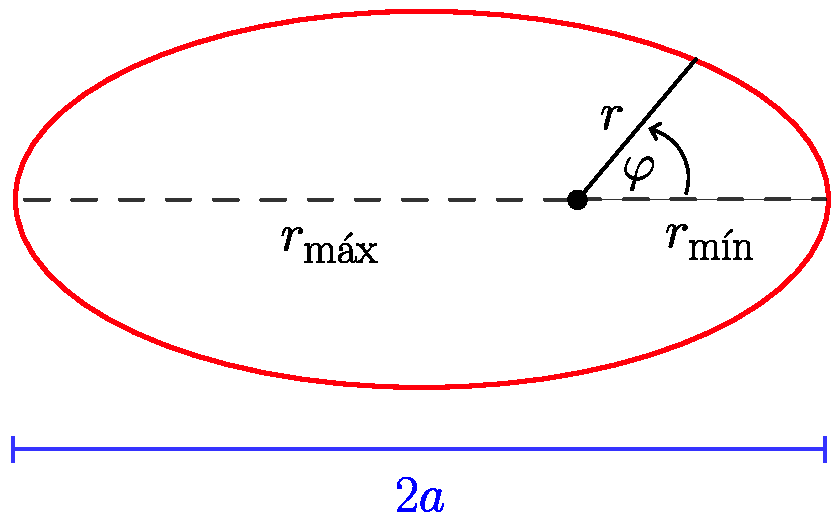
\includegraphics[scale=0.5]{Elipse}
\caption{Órbita elíptica.}
\label{fig:elipse}
\end{figure}

Para determinar los extremos locales de $u$, calculemos la primera derivada:
\begin{align}
u'(\varphi) &= \frac{1}{mh^2} \left[ - e(1-\epsilon)\sin[(1-\epsilon)\varphi] +  \frac{e^2\epsilon(1-\epsilon)}{3} \sin[2(1 - \epsilon)\varphi] \right] \nonumber\\
&=  \frac{1}{mh^2} \left[ - e(1-\epsilon)\sin[(1-\epsilon)\varphi] +  \frac{2 e^2\epsilon(1-\epsilon)}{3} \sin[(1 - \epsilon)\varphi] \cos[(1 - \epsilon)\varphi] \right] \nonumber \\
&= \frac{e(1-\epsilon)}{mh^2} \sin[(1-\epsilon)\varphi] \textcolor{red}{\left[-1 + \frac{2e\epsilon}{3} \cos[(1 - \epsilon)\varphi] \right]}.
\end{align}

Como $\epsilon \ll 1$, el término resaltado en rojo siempre es estrictamente negativo, entonces la derivada se anula en todo los $\varphi$ tales que
\begin{equation}
 \sin[(1-\epsilon)\varphi] = 0 \Leftrightarrow \varphi = \frac{k\pi}{1- \epsilon}, \quad k  \in \mathbb{Z}.
\end{equation}

La derivada de $u$ es positiva para $- \pi/(1 - \epsilon)<\varphi < 0$ ($u$ es creciente), negativa para $0 <\varphi < \pi/(1 - \epsilon)$ y positiva en $\pi/(1 - \epsilon) < \varphi < 2\pi/(1-\epsilon)$. Usando el criterio de la primera derivada para extremos locales,
\begin{align}
u_{\text{máx}} &= u(0) \nonumber\\
&= \frac{1}{mh^2} \left[ 1 + \epsilon \left( 1 + \frac{e^2}{2}\right) + e - \frac{\epsilon e^2}{6} \right] + \mathcal{O}(\epsilon^2) \nonumber \\
&= \frac{1}{mh^2} \left[ 1 + e + \epsilon \left( 1 + \frac{e^2}{3}\right) \right] + \mathcal{O}(\epsilon^2), \label{eq:u-max} \\
u_{\text{mín}} &= u\left(\frac{\pi}{1 - \epsilon}\right) \nonumber\\
&= \frac{1}{mh^2} \left[ 1 + \epsilon \left( 1 + \frac{e^2}{2}\right) - e + \frac{\epsilon e^2}{6} \right] + \mathcal{O}(\epsilon^2) \nonumber \\
&= \frac{1}{mh^2} \left[ 1 - e + \epsilon \left( 1 + \frac{2e^2}{3}\right) \right] + \mathcal{O}(\epsilon^2). \label{eq:u-min}
\end{align}

Reemplanzando \eqref{eq:u-max} y \eqref{eq:u-min} en \eqref{eq:semieje-mayor}:
\begin{align}
a &= \frac{u_{\text{máx}} + u_{\text{mín}}}{2 u_{\text{máx}} u_{\text{mín}}} \nonumber\\
&= \frac{\frac{1}{mh^2} \left[ 2 + \epsilon \left(2 + e^2 \right) \right] + \mathcal{O}(\epsilon^2)}{\frac{2}{m^2h^4} \left[(1+e)(1-e) + \epsilon (1+e) \left( 1 + \frac{2e^2}{3}\right) + \epsilon (1-e)\left(1  + \frac{e^2}{3}\right) \right]+ \mathcal{O}(\epsilon^2)}\nonumber \\
&= mh^2 \frac{2 + \mathcal{O}(\epsilon)}{2 (1-e^2) + \mathcal{O}(\epsilon)} \nonumber\\
&=  mh^2 \frac{2 + \mathcal{O}(\epsilon)}{2 (1-e^2)}  \frac{
1}{1 + \frac{\mathcal{O}(\epsilon)}{2(1-e^2)}} \nonumber\\
&= mh^2 \frac{2 + \mathcal{O}(\epsilon)}{2 (1-e^2)}   \left( 1 - \mathcal{O}(\epsilon) \right) \nonumber\\
&= \frac{mh^2}{1 - e^2} + \mathcal{O}(\epsilon).
\end{align}

Note que hemos expresado el semieje mayor a orden cero en $\epsilon$ porque lo calculamos de forma newtoniana (suponiendo que la órbita es una elipse).


Por lo tanto, a primer orden,
\begin{equation}
(\Delta \varphi)_{\text{rel}} \approx \frac{6\pi m}{a(1-e^2)}.
\end{equation}

Pero, $m = GM/c^2$. Entonces, en términos de la masa del cuerpo central:
\begin{shaded}
\begin{equation}
(\Delta \varphi)_{\text{rel}} \approx \frac{6\pi GM}{ac^2(1-e^2)}.
\end{equation}
\end{shaded}

Usando los mismos datos en \eqref{eq:mercury-data}, teniendo en consideración que la excentricidad de Mercurio es
\begin{equation}
e = 0.2056,
\end{equation}
la predicción relativista para el corrimiento del perihelio de Mercurio es 
\begin{equation}
(\Delta \varphi)_{\text{rel}} \approx \frac{6\pi (6.67430\times 10^{-11})(1.988 \times 10^{30})}{(57.909\times 10^{9})(299792458)^2(1 - 0.2056^2)} \frac{\text{rad}}{\text{rev}} \approx 5.018 \times 10^{-7} \ \text{rad}/\text{rev}. 
\end{equation}

Como $1\grad = 3600"$ (segundos de arco), tenemos que
\begin{equation}
\frac{\pi}{180} \ \text{rad} = 3600" \Rightarrow 1 \ \text{rad} = \left(\frac{648000}{\pi}\right)^{"}
\end{equation}

Así, 
\begin{equation}
(\Delta \varphi)_{\text{rel}} \approx (5.018 \times 10^{-7}) \left( \frac{648000}{\pi}\right) "/\text{rev} \approx 0.104 "/\text{rev}. 
\end{equation}

El periodo orbital de Mercurio es $T \approx 87.97 \,\text{días}$, si dividimos esta cantidad por $36500$, obtenemos que el periodo orbital es de $T \approx 2.41 \times 10^{-3} \,\text{siglos}$. Por lo tanto, el corrimiento del perihelio de Mercurio es 
\begin{shaded}
\begin{equation}
(\Delta \varphi)_{\text{rel}}  \approx 43.15 " / \text{siglo}.
\end{equation}
\end{shaded}
\end{document}
